%----------------------------------------------------------
% PACKAGES AND THEMES
%----------------------------------------------------------
\documentclass[aspectratio=169,xcolor=dvipsnames,handout]{beamer}

\usetheme{Darmstadt}
\usecolortheme{seahorse}

\usepackage[hangul]{kotex}
\usepackage{hyperref}
\usepackage{graphicx, array, adjustbox, makecell}
\usepackage{booktabs, multicol, multirow}
\setbeamercovered{transparent}

%----------------------------------------------------------
% TITLE PAGE
%----------------------------------------------------------
\title{쟁의조정 및 부당 노동행위}
\subtitle{노사관계의 이론과 실제}
\author{오성재}
\institute[CNU]
{\relax
    충남대학교 경제학과\\
}
\date{2024년 10월 7일}

%----------------------------------------------------------
\begin{document}
%----------------------------------------------------------

\frame{\titlepage}

\begin{frame}{목차}
    \small
    \tableofcontents
    %\tableofcontents[hideallsubsections]
\end{frame}

\section{쟁의조정}

\begin{frame}{쟁의조정}
    \begin{block}{쟁의조정}
        노사 쌍방이 자주적으로 해결하기 어렵고 쟁의로 인하여 사회전체의 질서와 안녕이 위태로울 때 부득이 국가 등 제3자가 협상타결을 위해 조력하는 것
    \end{block}
    \begin{itemize}[<+->]
        \item 쟁의조정제도에 지나치게 의존하면 노사 당사자들은 스스로 양보안을 내는 등의 적극적인 자세를 보이지 않음: 냉각효과 (chilling effect)
        \item 많은 노력이 수반되는 당사자간의 협상보다는 정부의 중재에 대한 의존도가 높아지게 됨: 중독효과 (narcotic effect)
        \begin{itemize}[<+->]
            \item 자주적 협상을 촉진하는 방법으로 파업의 가능성을 열어 두는 것이 가장 효과적. 당사자 스스로 해결책을 합의하는 것이 가장 지속적이고 효과적인 갈등해소 방안
        \end{itemize}
    \end{itemize}
\end{frame}

\subsection{쟁의조정의 유형}

\begin{frame}[allowframebreaks]{쟁의조정의 유형}
    \begin{enumerate}[<+->]
        \item 알선 (conciliation): 분쟁당사자를 설득하고 다시 화합하고 문제를 토론하게 하는 조정방법
        \begin{itemize}[<+->]
            \item 가장 간단한 쟁의조정 방법으로 분쟁의 중개자가 당사자와 만나 분쟁 해결방안 모색
            \item 알선자는 갈등해결안을 제시하지 않는 것이 일반적. 실효성에 문제가 있어 현행법에서 삭제 됨
        \end{itemize}
        \item 조정 (mediation): 조정자가 관계당사자의 의견 청취 후, 조정안을 작성하여 노사의 수락을 권고
        \begin{itemize}[<+->]
            \item 조정은 강제가 아니므로 조정안의 수락은 당사자들의 자유 의사임 
            \item 당사자의 흥분을 가라앉히고 이성적인 상태로 사태를 파악하도록 유도하여 비이성적 파업 방지
        \framebreak\relax
            \item 조정의 주요 기능
            \begin{itemize}[<+->]
                \item 쟁점사항에 대한 정보를 노사쌍방에게 제공하여 우발적 쟁의 억제 
                \item 당사자와 함께 쌍방이 받아들일 수 있는 해결책 모색
                \item 필요 시 어느 일방 또는 쌍방이 명예롭게 양보할 수 있도록 명분을 함께 탐색
                \item 갈등의 비용을 상승시킴으로써 갈등을 줄이는 방향으로 행동하도록 유도: 조정안을 어느 일방이 수용하거나 다른 일방이 거부할 경우 거부한 측이 여론의 질타를 받게 됨 을 주지시켜서 양측이 모두 조정안을 수용하도록 유도
            \end{itemize}
        \end{itemize}
        \item 중재 (arbitration): 준사법적 절차로 중재 결과를 관계당사자는 따라야 함 (구속)
        \begin{itemize}[<+->]
            \item 중재결정에 이의가 있을 경우 재심이나 행정소송 제기
        \end{itemize}
    \end{enumerate}
\end{frame}

\subsection{한국의 쟁의조정 및 중재제도}%

\begin{frame}{조정}
    \begin{block}{조정}
        노동위원회 내의 조정위원회가 관계당사자의 의견을 들어 조정안을 작성하여 노사의 수락을 권고
    \end{block}
    \begin{enumerate}[<+->]
        \item 조정대상: 이익분쟁 (권리분쟁 제외)
        \item 조정전치주의: 조정절차를 거치지 않으면 쟁의행위를 할 수 없음
        \begin{itemize}[<+->]
            \item 단체교섭이 결렬되면 당사자 일방의 신청에 의해 조정 개시
        \end{itemize}
        \item 조정과정: 노동쟁의 발생 사업장의 소재지 관찰 지방노동위원회가 조정 담당
        \begin{itemize}[<+->]
            \item 조정위원 선정 조정위원회는 사용자위원, 근로자위원, 공익위원 (위원장) 각 1명을 지명, 단 쌍방의 동의를 얻은 경우 단독 조정인을 두고 조정할 수 있음
            \item 조정기간 중 쟁의행위 금지: 일반사업 10일, 공익사업 15일
        \end{itemize}
    \end{enumerate}
\end{frame}

\begin{frame}[allowframebreaks]{공익사업의 쟁의조정}
    \begin{itemize}[<+->]
        \item 공익사업: 공중의 일상생활과 밀접한 관련이 있거나 국민경제에 미치는 영향이 큰 사업
        \begin{itemize}[<+->]
            \item 정기노선여객운수사업, 수도·전기·가스·석유정제 및 석유공급사업, 공중위생 및 의료사업, 은행 및 조폐사업, 방송 및 통신사업 
            \item 참고: 토지주택공사는 공기업이지만 일반사업장이고 하나은행은 사기업이지만 공익사업장임
        \end{itemize}
        \item 필수공익사업: 공익사업 중 그 업무의 중지 또는 폐지가 공중의 일상생활을 현저히 위태롭게 하거나 국민경제를 현저히 저해하고 그 업무의 대체가 용이하지 아니한 사업
        \begin{itemize}[<+->]
            \item 철도, 도시철도 및 항공운수사업, 수도·전기·가스·석유정제 및 석유공급사업, 병원 및 혈액공급사업, 한국은행사업, 통신사업
        \end{itemize}
        \item 공익사업에 대한 조정절차상의 특칙
        \begin{itemize}[<+->]
            \item 현행법상 일반사업과는 절차가 상이
            \item 관계당사자 일방에 의한 조정신청 시 15일간 쟁의행위 금지 (일반사업은 10일)
            \item 공익사업의 쟁의조정은 특별조정위원회에서 담당하며 공익대표 위원으로 구성
            \item 긴급조정을 행할 수 있음
            \item 단, 필수공익사업은 강제중재 실시, 중재기간 중 15일간 쟁의행위 금지
        \end{itemize}
    \end{itemize}
    \begin{table}
        \centering
        \resizebox{.8\textwidth}{!}{\relax
            \begin{tabular}{p{5cm}|p{5cm}|p{5cm}}
\toprule
일반사업장 & 공익사업장 & 필수공익사업장 \\
\midrule
쟁의전 10일간 조정 & 쟁의전 15일간 조정  & 쟁의전 15일간 조정         \\
                   & 특별조정위원회 구성 & 특별조정위원회 구성        \\
                   & 긴급조정적용 가능   & 긴급조정적용 가능          \\
                   &                     & 파업중 필수유지업무 지정   \\
                   &                     & 파업인력 절반까지 대체가능 \\
\bottomrule
\end{tabular}

        }
        \caption{쟁의권 제한}
    \end{table}
\end{frame}

\begin{frame}[allowframebreaks]{긴급조정}
    \begin{block}{긴급조정}
        쟁의행위가 공익사업에 관한 것이거나 그 규모가 크고 중대한 것으로서 국민경제나 국민의 일상생활을 위태롭게 할 위험이 있는 경우, 고용노동부장관의 결정에 의하여 강제적으로 조정 개시
    \end{block}
    \begin{enumerate}[<+->]
        \item 요건: 실질적 및 형식적 요건 충족
        \begin{itemize}[<+->]
            \item 실직적 요건
            \begin{itemize}[<+->]
                \item 공익사업에 관한 것이거나, 그 규모가 크거나, 그 성질이 특별한 것이어야
                \item 국민경제를 해하거나, 국민의 일상생활을 위태롭게 한 위험이 현존하여야
            \end{itemize}
            \item 형식적 요건
            \begin{itemize}[<+->]
                \item 고용노동부장관이 중앙노동위원회 위원의 의견 청취 후 긴급조정 결정
            \end{itemize}
        \end{itemize}
        \item 절차: 중앙노동위원회는 통보받은 후 즉시 조정 개시 조정의 불가능 시 중재 회부 결정
        \begin{itemize}[<+->]
            \item 지체 없이 그 이유를 붙여 공표, 중노위 및 관계당사자에 통보
            \item 조정의 불가능 시: 긴급조정 결정통보 15일 이내에 중재에의 회부 여부 결정
            \item 중재 회부 결정 시: 지체 없이 중재 개시
        \end{itemize}
        \item 쟁의행위 금지: 긴급조정 공표 후, 쟁의행위의 즉시 중지 및 30일간 쟁의행위 금지
        \item 효과: 관계당사자가 수락한 조정안 또는 중재결정은 단체협약과 동일한 효력 가짐
    \end{enumerate}
\end{frame}

\section{부당노동행위}%

\subsection{부당노동행위의 의의와 특색}%

\begin{frame}[allowframebreaks]{부당노동행위}
    \begin{block}{부당노동행위 (unfair labor practice)}
        노동3권의 구체적인 보장을 위한 행정적인 구제제도
    \end{block}
    \begin{itemize}[<+->]
        \item 제도화 이유
        \begin{itemize}[<+->]
            \item 사법적 구제절차는 오랜 시일과 비용이 많이 듦
            \item 급변하는 고용관계에 효과적인 대응 미흡
            \item 사법적 심사를 조건으로 하는 행정기관에 의한 구제방법을 채택함으로써 고용관계에 신속하게 대처하고자 함
        \end{itemize}
    \framebreak\relax
    \item 부당노동행위의 역사
        \begin{itemize}[<+->]
            \item 1935년 미국의 Wagner 법에서 처음으로 창설
            \item ILO조약 제98조: 부당노동행위제도의 창설 요구
            \item 「노동조합 및 노동관계조정법』제81조 이하에서 각각 규정하고 있음
            \item 미국에서는 노사 양측의 부당노동행위를 규정하고 있으나 우리나라에서는 사용자의 부당노동행위만을 규정하고 있음
        \end{itemize}
    \end{itemize}
\end{frame}

\subsection{부당노동행위의 종류와 요건}%

\begin{frame}[allowframebreaks]{불이익대우}
    \begin{itemize}[<+->]
        \item 불이익 대우의 원인
        \begin{itemize}[<+->]
            \item 근로자가 노동조합에 가입 또는 가입하려고 하였거나 기타 노동조합의 업무를 위한 정당한 행위를 한 것을 이유로 그 근로자를 해고하거나 그 근로자에게 불이익을 주는 행위
            \item 근로자가 정당한 단체행위에 참가한 것을 이유로 하거나 또는 노동위원회에 대하여 사용자가 이 조의 규정에 위반한 것을 신고하거나 그에 관한 증언을 하거나 기타 행정관청에 증거를 제출한 것을 이유로 그 근로자를 해고하거나 그 근로자에게 불이익을 주는 행위.
            \item 정당한 노조활동: 단체교섭, 쟁의행위 및 조합간부 선거·발언·결의·업무출장 등
        \end{itemize}
    \item 유형: 해고나 전근, 배치전환, 출근정지, 휴직, 복직거부, 계약갱신 거부, 고용거부, 차별승급, 강등 및 복지시설의 차별적 이용, 공장폐쇄 등
    \item 단, 사용자의 불이익대우와 피고용인의 조합활동 사이에 인과관계가 있어야 함 (객관적 합리적 추정)
    \end{itemize}
\end{frame}

\begin{frame}{황견계약}
\begin{block}{황견계약 (yellow-dog contract)}
        근로자가 어느 노동조합에 가입하지 아니할 것 또는 탈퇴할 것을 고용조건으로 하거나 특정한 노동조합의 조합원이 될 것을 고용조건으로 하는 행위
    \end{block}
    \begin{exampleblock}{『노동조합 및 노동관계조정법』제81조 제2호}
        \begin{itemize}[<+->]
            \item 노동조합을 가입하지 않거나 탈퇴할 것
            \item 조합에 가입하더라도 조합활동을 하지 말 것
            \item 어용조합에의 가입
        \end{itemize}
    \end{exampleblock}
    \begin{itemize}[<+->]
        \item 단, 우리나라의 경우 유니온숍은 황견계약이라는 부당노동행위에 해당되지 않는다는 특칙을 두고 있음
    \end{itemize}
\end{frame}

\begin{frame}[allowframebreaks]{단체교섭의 거부}
    \begin{itemize}[<+->]
        \item 단체교섭의 거부: 노동조합의 대표자 또는 노동조합으로부터 위임을 받은 자와의 단체협약 체결 기타 단체교섭을 정당한 이유없이 거부하거나 해태하는 행위
        \begin{itemize}[<+->]
            \item 타당한 장소와 시간임에도 불구하고 사용자대표가 출석하지 않는 경우
            \item 이유 없이 대안을 제시하지 않는 경우
            \item 쟁의에 대한 사실을 왜곡하여 상대방을 혼란시키는 경우
            \item 최종단계에서 협약의 체결을 거부하는 경우
        \end{itemize}
    \framebreak\relax
    \item 정당한 이유에 의한 거부행위
        \begin{itemize}[<+->]
            \item 교섭권한이 없는 사용자의 하부조직에서의 단체교섭 거부
            \item 경영권에 대한 교섭의 거부
            \item 협약기간 중에 그의 개정을 요구하는 단체교섭의 거부
            \item 노조측의 교섭담당자가 부당하게 많은 경우
            \item 지나치게 장기화하거나 폭행·협박을 수반하거나 연금상태 하에서의 단체교섭 거부
        \end{itemize}
    \end{itemize}
\end{frame}

\begin{frame}{지배, 개입 및 경비원조}
    \begin{itemize}[<+->]
        \item 근로자가 노동조합의 조직 또는 운영하는 것을 지배하거나 이에 개입하는 행위와 노동조합의 전임자에게 급여를 지원하거나 노동조합의 운영비를 원조하는 행위,
        \begin{itemize}[<+->]
            \item 다만 근로자가 근로시간 중에 사용자와 협의 또는 교섭하는 것을 사용자가 허용함은 무방하며 또한 근로자의 후생자금 또는 경제상의 불행 기타 재액의 방지와 구제 등을 위한 기금의 기부와 최소한의 규모의 노동조합 사무소의 제공은 예외로 함
        \end{itemize}
        \item 경비원조의 예
        \begin{itemize}[<+->]
            \item 조합운영비의 지급, 조합간부의 출장비 지급, 조합대회의 경비 원조, 쟁의행위 기간중의 임금상당액의 지급
        \end{itemize}
    \end{itemize}
\end{frame}

\subsection{부당노동행위의 구제제도}

\begin{frame}[allowframebreaks]{구제절차}
    \centering
    \begin{figure}
        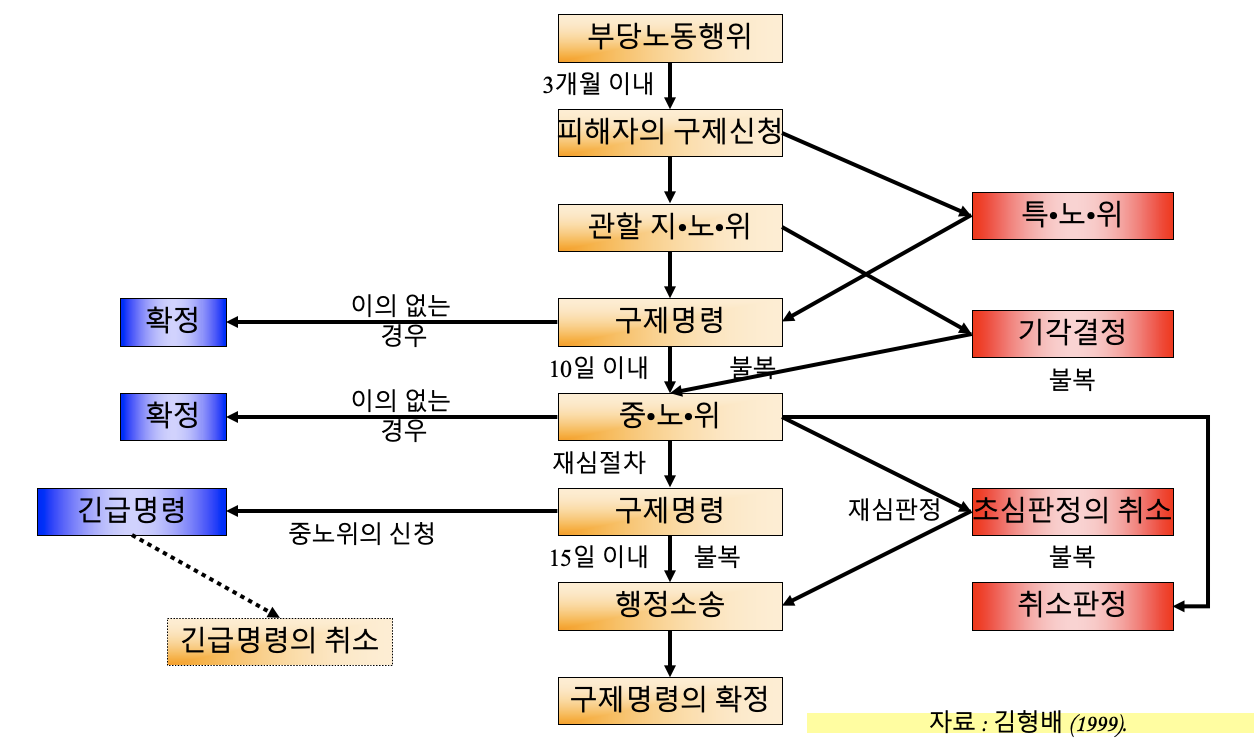
\includegraphics[width=.6\textwidth]{pic/구제제도.png}
        \caption{부당노동행위의 구제절차}
    \end{figure}
    \begin{itemize}[<+->]
        \item 구체신청: 권리를 침해당한 피고용인 또는 노동조합이 노동위원회에 부당노동행위 신고
        \item 노동위원회 심사: 2심제 원칙
        \begin{itemize}[<+->]
            \item 1심 (지방노동위원회), 2심 (중앙노동위원회)
        \end{itemize}
        \item 지노위에서 부당노동행위가 성립되면 구제명령, 그렇지 않으면 기각
        \begin{itemize}[<+->]
            \item 지노위의 판정에 불복하면 명령서 또는 결정서를 받은 지 10일 내에 중앙노동위에 재심판정 신청
            \item 중앙노동위의 재심판정에 이의가 있으면 결정서를 받은 지 15일 내에 행정소송 (3심제) 제기 가능
        \end{itemize}
    \item 구제명령이 확정되면 사용자는 구제명령을 이행하여야 하고 불이행 시 벌칙
    \end{itemize}
\end{frame}

\subsection{부당노동행위의 신청 및 구제현황}

\begin{frame}{최근 현황}
    \begin{itemize}[<+->]
        \item 부당노동행위 신청건수
        \begin{itemize}[<+->]
            \item 1989년 최다 발생 이후 감소세, 경제위기 (1998년) 이후 다시 증가세
            \item 2001년 이후 다시 하락세, 2010년이후 900여건으로 유지
        \end{itemize}
        \item 파업발생추이와 흡사한 양상을 보이고 있음: 파업 시 노조가 사용자를 압박하기 위해 신청을 하였기 때문
    \end{itemize}
\end{frame}

%------------------------------------------------
\end{document}
%------------------------------------------------
